\begin{figure*}[t]
    \centering
    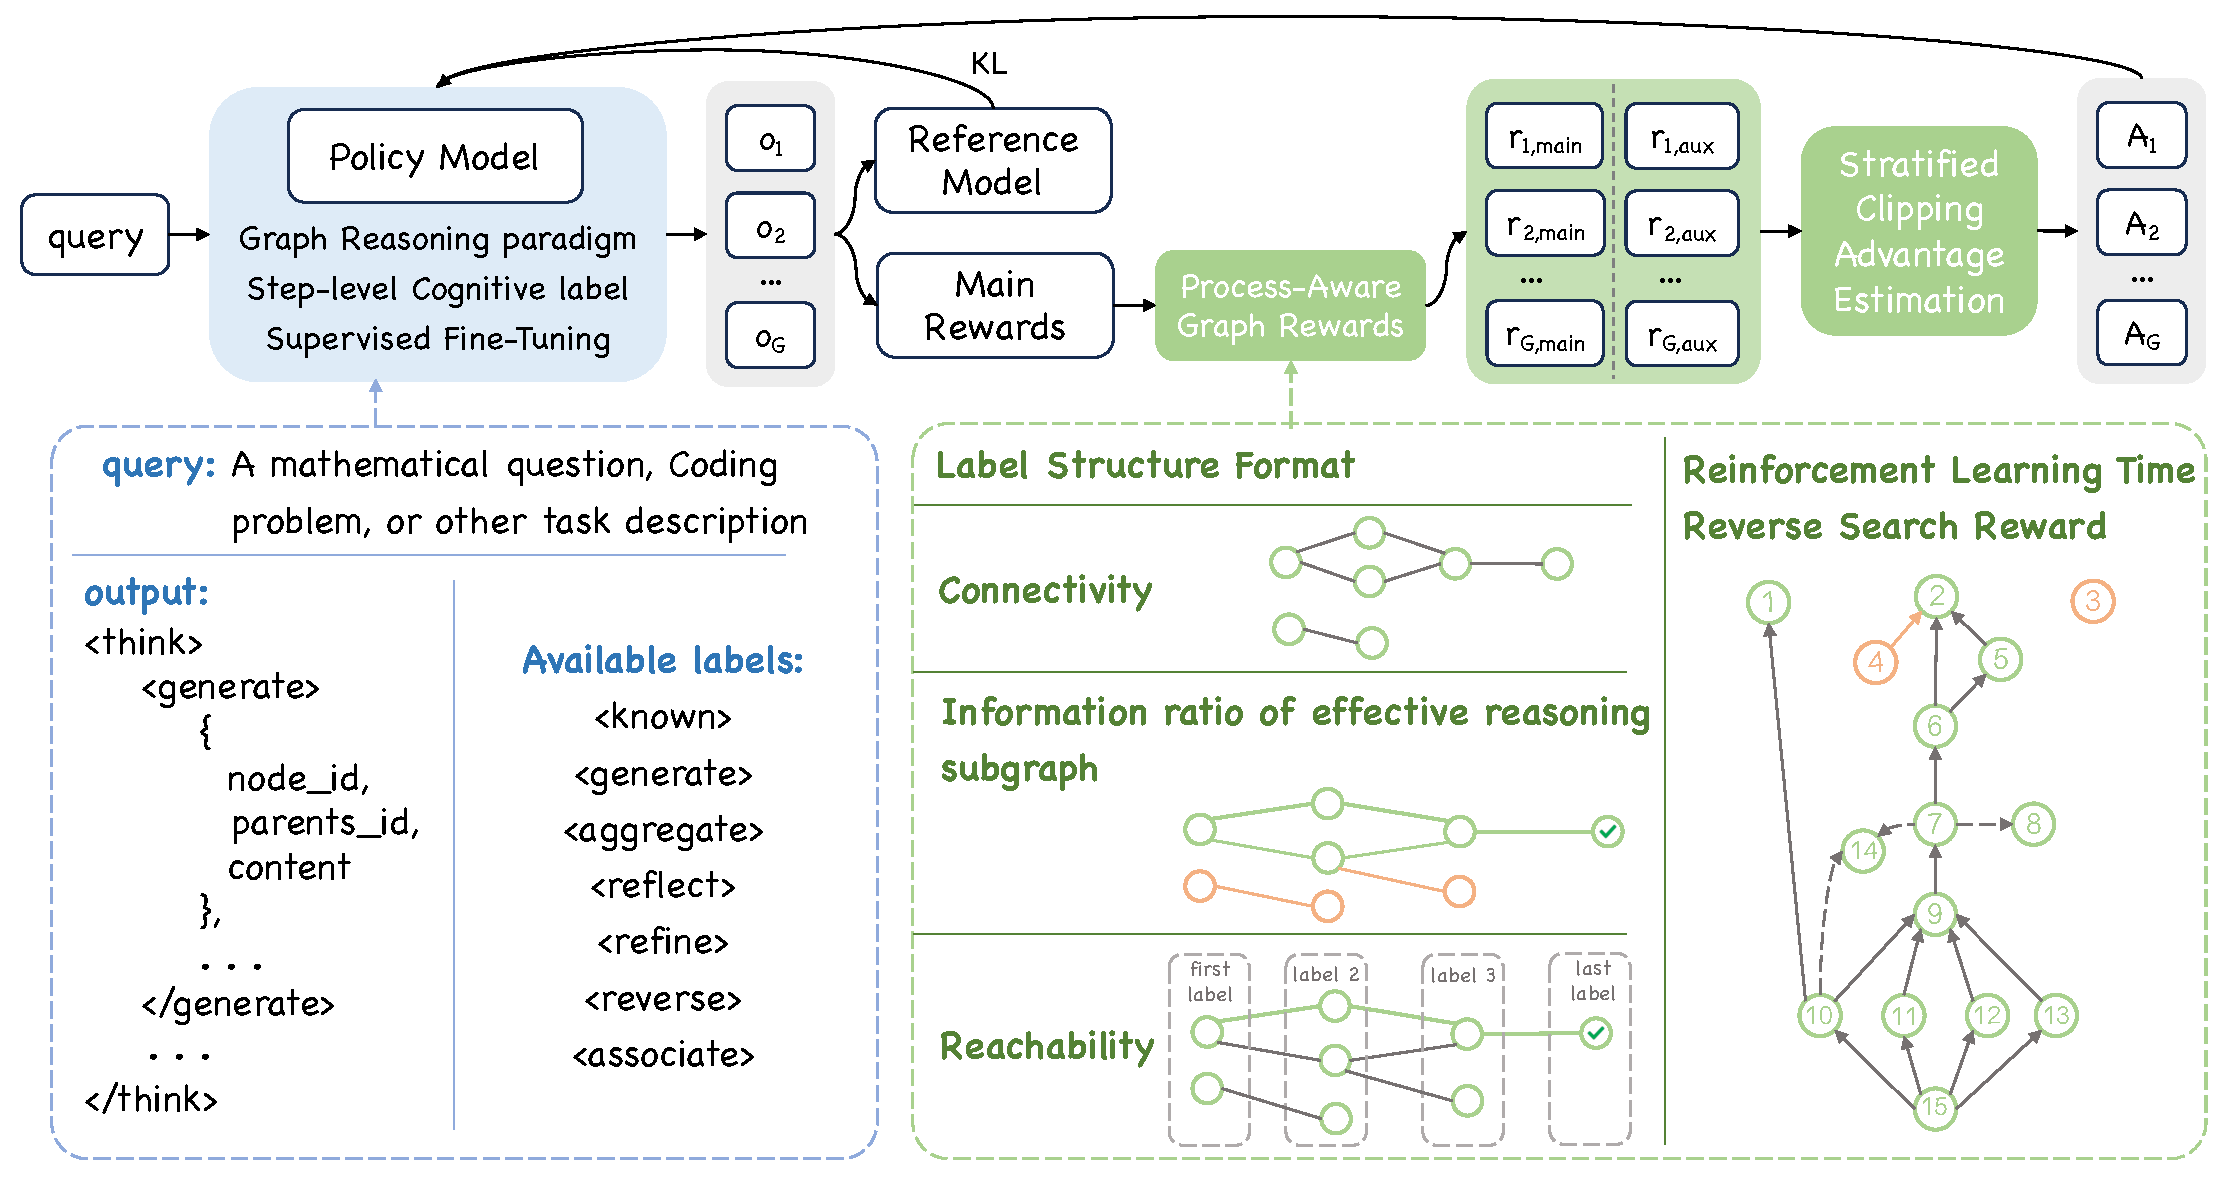
\includegraphics[width=\linewidth]{Figures/framework-v6.pdf}
    \caption{
    Overview of the proposed method.
    }
    \label{fig:overview}
\end{figure*}

As illustrated in Figure~\ref{fig:overview}, our method consists of two main components:
\begin{itemize}
    \item \textbf{Graph Reasoning Paradigm}, which enables LLMs to produce symbolized, interpretable, verifiable, and accurate graph-structured reasoning through supervised fine-tuning; 
    \item \textbf{PASC-GRPO}, a reinforcement learning framework that incorporates process-aware graph rewards and stratified clipping advantage estimation to further improve reasoning quality and training stability.
\end{itemize}

\subsection{Graph Reasoning Paradigm}
\label{sec:grp}

We design a graph-structured reasoning paradigm in which the model directly outputs its reasoning process as a graph.
This paradigm is realized through step-level cognitive labels, node-based reasoning representation, and data synthesis followed by supervised fine-tuning (SFT).

\subsubsection{Step-level Cognitive Labels}
\label{sec:labels}

Existing large reasoning models employ only coarse-grained \texttt{<think>} and \texttt{<answer>} tags, without further decomposition of the reasoning process.
As a result, emergent operations such as reflection may occur at arbitrary stages and with inconsistent content during reasoning.
To address this limitation, we introduce step-level reasoning tags.
Details are provided in Appendix~\ref{app:labels_description}.

By explicitly selecting a cognitive label at each step, the model is encouraged to reason about \emph{how} to emerge, not only \emph{can} emerge, which improves the interpretability of the reasoning process and the reliability of utilizing different reasoning patterns.

\subsubsection{Node-based Reasoning Representation}
\label{sec:nodes}

Under the graph reasoning paradigm, each cognitive label wraps one or more reasoning nodes.
Each node is defined as a tuple:
\begin{equation}
v = (\textit{id}, \textit{parents\_id}, \textit{content}),
\end{equation}
where \textit{id} is the unique identifier of the node, \textit{parents\_id} is a list of parent node ids, and \textit{content} denotes the content of the reasoning step.

This node-based representation enables the reasoning process to be abstracted into a directed graph, which forms the foundation for graph-structured, process-aware optimization.

\subsubsection{Data Synthesis and SFT}
\label{sec:data_sft}

% \subsubsection{Iterative Graph-Augmented Synthesis}

To enhance the model's structural reasoning while maintaining its inherent inference fluidity, we implement an iterative synthesis pipeline. This process consists of three primary stages:

\paragraph{Generating and Validating Reasoning Traces.}
For each problem $p$ in the dataset $\mathcal{P}$, we first sample a reasoning trace using a teacher LLM $\mathcal{T}$ and verify its final answer against the ground truth.
If the answer is correct, the trace is retained for subsequent graph-structured transformation.
If the answer is incorrect, we trigger a regeneration process with an upper bound on the number of retries.
This regeneration continues until either a correct reasoning trace is obtained or the maximum retry limit is reached.
Only reasoning traces with verified correct answers are passed to the next stage.

\paragraph{Graph-Structured Translation.}
Given a validated reasoning trace $T$, we translate it into the Graph Reasoning Paradigm. This translation explicitly exposes the latent reasoning structure while preserving the original semantic content of the trace.
Graph representations derived from originally correct and regenerated traces are jointly collected for quality inspection. Detailed prompts and examples are provided in Appendix~\ref{app:translation}.

\paragraph{Graphical CoT Verification and Refinement.}
To ensure the quality of the synthesized graph-structured reasoning data, we introduce an automated quality control loop that evaluates each generated graph from two complementary aspects:

\begin{itemize}
    \item \textbf{Node--Label Consistency.}
    We verify that the reasoning content of each node conforms to the semantic scope of its assigned label.

    \item \textbf{Parent--Child Coherence.}
    We check whether each node is logically coherent with its parent node(s), ensuring a consistent and non-contradictory reasoning flow.
\end{itemize}

If a graph $G$ fails either of the above checks, we generate structured feedback that explicitly identifies the problematic nodes and the corresponding violation types.
This feedback, together with a predefined refinement prompt template, is fed back to the LLM to trigger a re-translation step.
The refinement process iterates until the graph passes all quality checks or a maximum number of translation attempts is reached. 
Detailed prompts and cases are provided in Appendix~\ref{app:verify}.

\paragraph{Supervised Fine-Tuning with Mixed Reasoning Formats.}  
After constructing the graph-structured reasoning dataset, we perform supervised fine-tuning on both graph-structured traces and a subset of original CoT traces that could not be converted into valid graphs. Although these samples do not conform to the graph format, their problem–solution pairs and coherent reasoning steps remain informative. This mixed-format training allows the model to internalize the graph reasoning paradigm while preserving fluency, completeness, and generalization of its native reasoning behavior.


\subsection{PASC-GRPO}
\label{sec:pasc_grpo}

Fine-grained control over the reasoning process is crucial for solving complex reasoning tasks. \cite{Shao2025DeepSeekMathV2TS}
After SFT, the model internalizes the graph reasoning paradigm, where the reasoning process can be abstracted as a graph independent of specific reasoning content.
Building on it, we propose \textbf{PASC-GRPO} (\textbf{P}rocess-\textbf{A}ware \textbf{S}tratified \textbf{C}lipping GRPO), which enables optimization of reasoning length and process quality.

\subsubsection{Process-Aware Graph Rewards}
\label{sec:graph_rewards}

We use NetworkX~\cite{SciPyProceedings_11} to construct reasoning graphs.
On this basis, we design \emph{Process-Aware Graph Rewards}, which can be grouped into three categories:

\begin{itemize}
    \item \textbf{Graph structure format rewards}, including the \emph{Label Structure Format Reward}, which enforce valid and well-formed reasoning graphs.
    \item \textbf{Reasoning length rewards}, including the \emph{Connectivity Reward}, which encourages fewer connected components, and the \emph{Information Ratio of Effective Reasoning Subgraph}, which promotes shorter reasoning paths within each component.
    \item \textbf{Reasoning process quality rewards}, including the \emph{Reachability Reward} at the global process level, and the \emph{Reinforcement Learning Time Reverse Search Reward} at the step level.
\end{itemize}

\paragraph{Label Structure Format Rewards.}
We introduce it to enforce the structural validity of graph-structured reasoning.
Let $\mathcal{G}=(\mathcal{V}, \mathcal{E})$ denote the reasoning graph, where $Pa(v)$ is the set of parent nodes of $v$.
Let $\mathcal{K}$, $\mathcal{A}$, and $\mathcal{R}$ denote \textit{known}, \textit{aggregate}, and \textit{refine} nodes, and $\mathcal{T}$ denote the set of reasoning tags. The overall format reward $R_{fmt}$ is defined as the average of three complementary sub-rewards:
\begin{equation}
R_{fmt}
=
\frac{1}{3}
\left(
R_{dens}
+
R_{topo}
+
R_{para}
\right).
\end{equation}

\begin{itemize}

\item \textbf{Node Density.}
For \textit{aggregate} and \textit{refine}, each tag is required to wrap exactly one node:
\begin{equation}
R_{dens}
=
\frac{1}{|\mathcal{A} \cup \mathcal{R}|}
\sum_{v \in \mathcal{A} \cup \mathcal{R}}
\mathds{1}
\big(
|v|_{\text{label}} = 1
\big).
\end{equation}

\item \textbf{Topological Validity.} Specifically, \textit{known} nodes must not depend on prior reasoning, \textit{aggregate} nodes must combine multiple predecessors, and \textit{refine} nodes must extend exactly one preceding step:
\begin{equation}
R_{topo}
=
\frac{1}{|\mathcal{K} \cup \mathcal{A} \cup \mathcal{R}|}
\sum_{v \in \mathcal{K} \cup \mathcal{A} \cup \mathcal{R}}
\Phi(v),
\end{equation}
\begin{equation}
\Phi(v)
=
\begin{cases}
1, & |Pa(v)| = 0,\ v \in \mathcal{K}, \\
1, & |Pa(v)| > 1,\ v \in \mathcal{A}, \\
1, & |Pa(v)| = 1,\ v \in \mathcal{R}, \\
0, & \text{otherwise}.
\end{cases}
\end{equation}


\item \textbf{Parallelism.}
Nodes within a tag are treated as parallel reasoning units and are therefore prohibited from forming parent--child relations:
\begin{equation}
\begin{aligned}
R_{para}
&=
\frac{1}{|\mathcal{T}|}
\sum_{T \in \mathcal{T}}
\mathds{1}
\Big(
\forall\, v_i, v_j \in T, \\
&\qquad
v_i \notin Pa(v_j)
\Big)
\end{aligned}
\end{equation}
\end{itemize}

\paragraph{Connectivity Reward.} To discourage fragmented reasoning, we define the connectivity reward based on the number of connected subgraphs:
\begin{equation}
R_{conn}
=
\frac{1}{n},
\end{equation}
where $n$ is the number of connected subgraphs in $\mathcal{G}$. This reward favors reasoning with fewer isolated branches, resembling more focused reasoning.

\paragraph{Information Ratio of Effective Reasoning Subgraph.}
We define the effective reasoning subgraph (ERS) as the part of the reasoning graph that effectively contributes to reaching the final answer.
The shortest path from the initial conditions to the answer node forms a backbone of effective reasoning.
Reasoning branches that diverge from this backbone but eventually merge back are also considered effective.
Branches that do not reconnect are treated as ineffective explorations, as they may correspond to incorrect reasoning attempts.
\begin{equation}
\mathcal{V}_{ERS}
=
\{\, v \in \mathcal{V} \mid v_{start} \rightsquigarrow v \rightsquigarrow v_{end} \,\}.
\end{equation}

The ERS Information Ratio $R_{ers}$ is measured by token count $I(\cdot)$:
\begin{equation}
    R_{ent} = \frac{\sum_{v \in \mathcal{V}_{ERS}} I(v)}{\sum_{v \in \mathcal{V}_{Total}} I(v)}
\end{equation}
This encourages the model to avoid "dead-end" branches and redundant chatter.

\begin{figure*}[t]
    \centering
    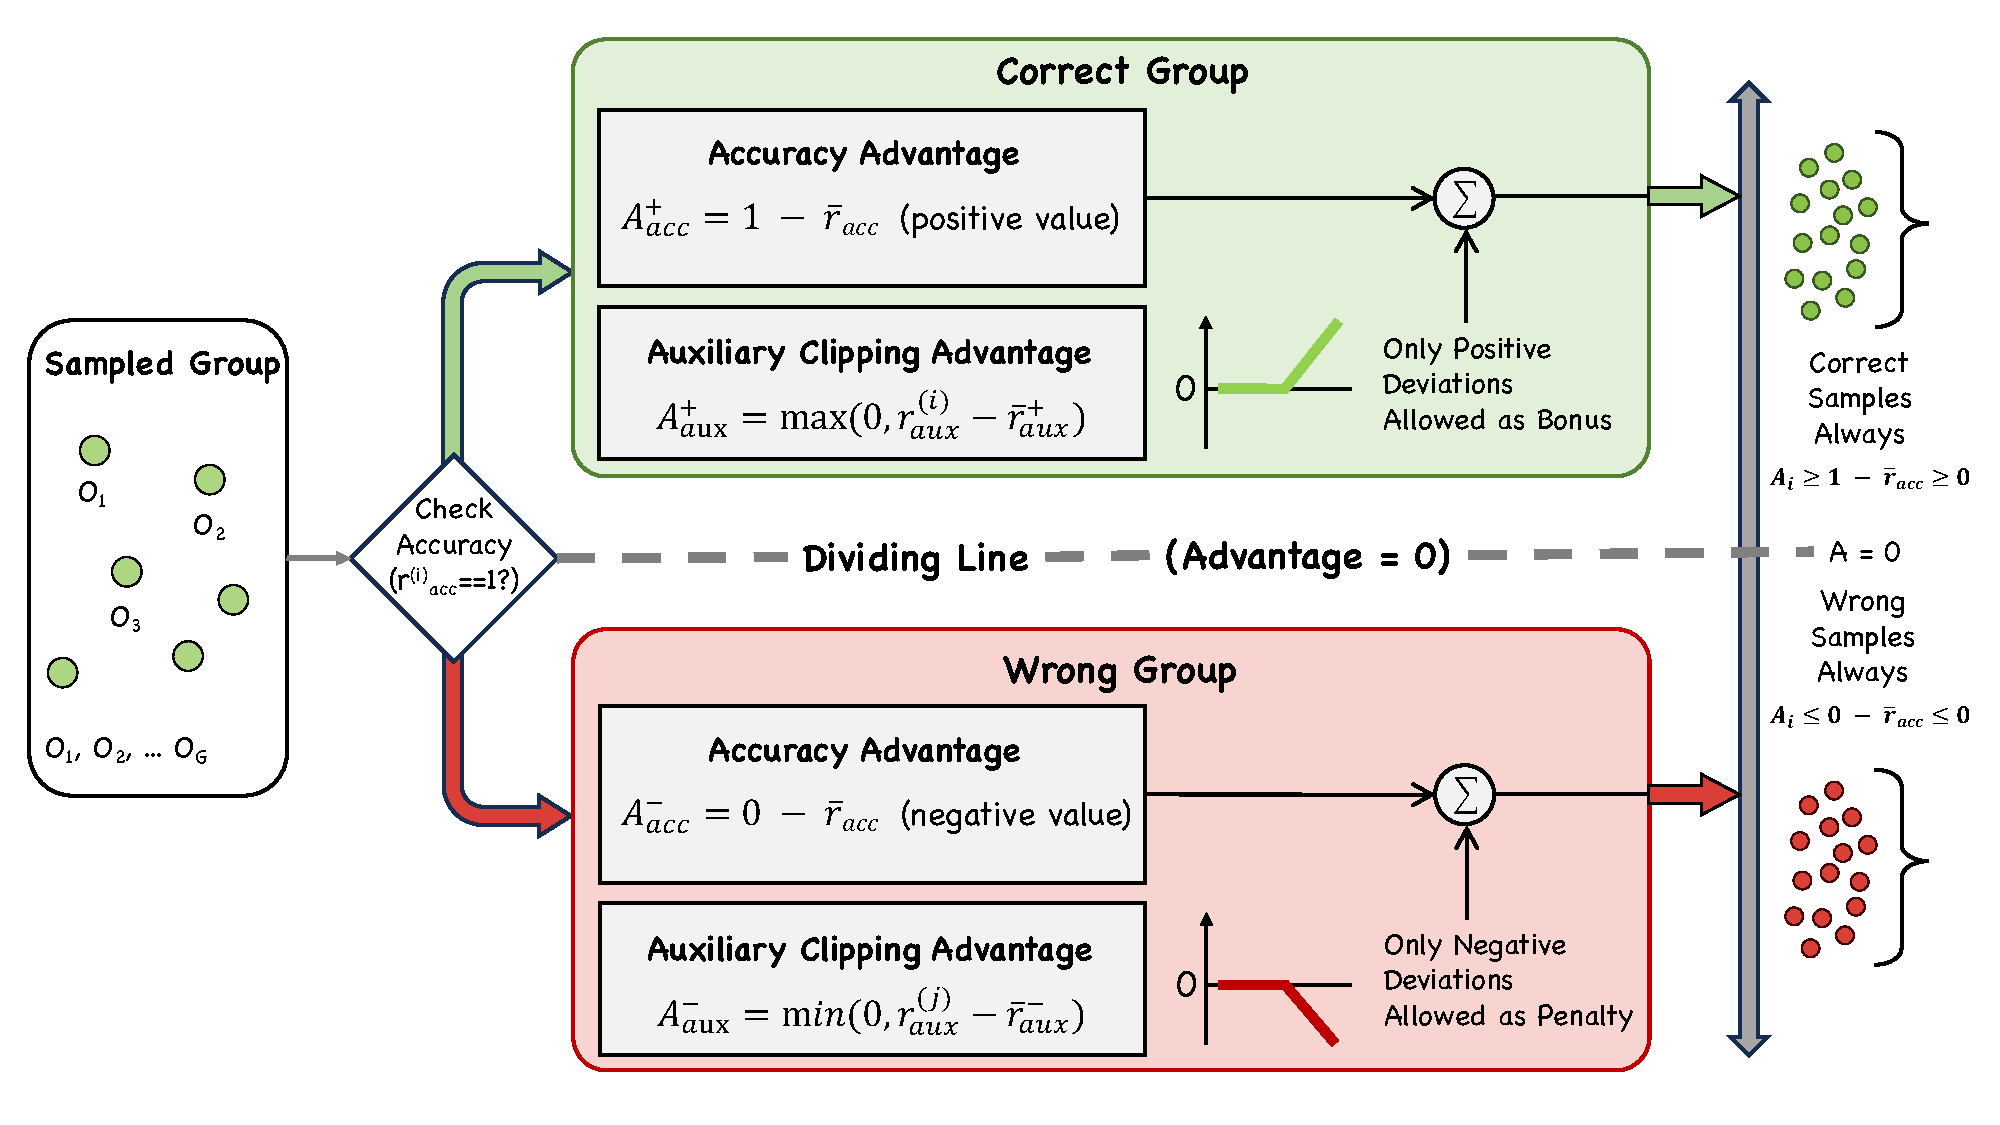
\includegraphics[width=\linewidth]{Figures/SCAE_v2.pdf}
    \caption{
    Illustration of the Stratified Clipping Advantage Estimation.
    }
    \label{fig:scae}
\end{figure*}

\paragraph{Reachability Reward.}
To mitigate the "wrong process, correct answer" phenomenon \cite{Akter2025InducingFI}, we evaluate the end-to-end logical flow:
\begin{equation}
R_{reach} = \mathds{1}(v_{start} \rightsquigarrow v_{end})
\end{equation}
where $R_{reach} = 1$ if there exists a directed path in $\mathcal{G}$, ensuring the reasoning process is complete and leads to the final answer.

\paragraph{Reinforcement Learning Time Reverse Search Reward.}
Unlike forward heuristics such as MCTS or PRM, which incrementally expand reasoning paths to approximate the correct answer, our reward directly leverages the known answer. 
After the reasoning graph $\mathcal{G}$ is completed, we traverse it backward from the answer node $v_{ans}$ to identify which nodes actually contribute to reaching the answer.For each node $v \in \mathcal{V}$, we assign
\begin{equation}
r(v) =
\begin{cases}
1 & \text{if } v \rightsquigarrow v_{ans}, \\
0 & \text{otherwise,}
\end{cases}
\end{equation}
where $v \rightsquigarrow v_{ans}$ indicates that $v$ is reachable from $v_{ans}$ via backward traversal.
The total reward is computed as the average over all nodes:
\begin{equation}
R_{rev} = \frac{1}{|\mathcal{V}|} \sum_{v \in \mathcal{V}} r(v).
\end{equation}

\paragraph{Overall Process-Aware Graph Reward.}
The final process-aware graph reward is defined as a weighted sum with scalar weights $w_1,\dots,w_5$, where each component reward is normalized to $[0,1]$ and $\sum_{i=1}^{5} w_i = 1$:

\begin{equation}
\begin{aligned}
R_{\text{graph}}
&=
w_1 R_{fmt}
+ w_2 R_{conn}
+ w_3 R_{ers} \\
&\quad
+ w_4 R_{reach}
+ w_5 R_{rev}
\end{aligned}
\end{equation}

\subsubsection{Stratified Clipping Advantage Estimation}

To mitigate the reward hacking phenomenon — where the model might optimize graph-structured rewards despite producing incorrect answers — we propose the \textbf{Stratified Clipping Advantage Estimation} (SCAE) method. This approach hierarchically prioritizes task accuracy over auxiliary structural signals. The logical flow of the proposed SCAE is illustrated in Figure \ref{fig:scae}.

\paragraph{Group Stratification.}
For a sampled group of $G$ reasoning traces, we first calculate the mean accuracy reward $\bar{r}_{acc} \in [0, 1]$. The group is then partitioned into a \textbf{Correct Group} ($\mathcal{G}_{corr}$) where $r_{acc}^{(i)}=1$ and a \textbf{Wrong Group} ($\mathcal{G}_{wrong}$) where $r_{acc}^{(j)}=0$. We define the baseline accuracy advantages for these strata as:
\begin{equation}
    A_{acc} = 
    \begin{cases} 
    1 - \bar{r}_{acc}, & \text{if } i \in \mathcal{G}_{corr} \\
    0 - \bar{r}_{acc}, & \text{if } j \in \mathcal{G}_{wrong}
    \end{cases}
\end{equation}
This ensures the baseline advantage is non-negative ($A_{acc} \ge 0$) for the correct group and non-positive ($A_{acc} \le 0$) for the wrong group.

\paragraph{Asymmetrical Auxiliary Clipping.}  
Within each stratum, we calculate the mean of the auxiliary graph rewards, denoted as $\bar{r}_{aux}^+$ for the correct group and $\bar{r}_{aux}^-$ for the wrong group. Here, the auxiliary reward refers to all rewards other than the main reward (e.g. accuracy reward), such as graph or format rewards. To prevent structural rewards from overriding the accuracy signal, we apply asymmetrical clipping:

\begin{itemize}
    % \setlength{\itemsep}{2pt}   % 每一项之间的垂直间距
    % \setlength{\parskip}{0pt}   % 每一项段落间距
    % \setlength{\parsep}{0pt}    % 段落之间的额外间距
  
    \item \textbf{Correct Group Clipping:} In $\mathcal{G}_{corr}$, structural rewards are treated strictly as bonuses. Even if a trace's structural reward $r_{aux}^{(i)}$ is below the group mean, it is not penalized, ensuring the final advantage $A_i$ never falls below the accuracy baseline:
    \begin{equation}
        A_i = (1 - \bar{r}_{acc}) + \max(0, r_{aux}^{(i)} - \bar{r}_{aux}^+)
    \end{equation}
    to ensure $i \in \mathcal{G}_{corr}$, $A_i \ge 1 - \bar{r}_{acc} \ge 0$.

    \item \textbf{Wrong Group Clipping:} In $\mathcal{G}_{wrong}$, structural rewards serve exclusively as penalties. No matter how high the structural quality $r_{aux}^{(j)}$ is relative to the mean, it receives no credit, ensuring the advantage remains non-positive:
    \begin{equation}
        A_j = (0 - \bar{r}_{acc}) + \min(0, r_{aux}^{(j)} - \bar{r}_{aux}^-)
    \end{equation}
    to ensure $j \in \mathcal{G}_{wrong}$, $A_j \le 0 - \bar{r}_{acc} \le 0$.
\end{itemize}

In summary, SCAE offers the following advantages for training graph-reasoning models:

\begin{table*}[htbp]
    \centering
    \caption{Experimental results on Mathematical Reasoning and Code Generation benchmarks.}
    \label{tab:main_results}
    \small
    \renewcommand{\arraystretch}{1.2} % 增加行间距，提升阅读舒适度
    \begin{tabular}{lccccc}
        \toprule
        % --- 数学推理分类标题 (灰色底色) ---
        \rowcolor{gray!15}
        \multicolumn{6}{c}{\textbf{Mathematical Reasoning}} \\
        \midrule
        \textbf{Model} & \textbf{GSM8K} & \textbf{MATH500} & \textbf{AMC23} & \textbf{AIME24} & \textbf{AIME25} \\
        \midrule
        LLaMA-3.1-8B-Instruct & 85.00 & 54.80 & 41.20 & 6.30 & 2.70  \\
        Gemma-3-12B-IT         & 94.40 & 85.60 & 77.30 & 22.40 & 18.80  \\
        Gemma-3-27B-IT         & \textbf{95.90} & 90.00 & 80.50 & 32.60 & 24.00  \\
        \midrule
        Qwen3-4B-Base               & 70.20 & 55.43 & 19.17 & 10.00 & 6.33  \\
        \rowcolor{cyan!5} % 方法行 (浅青色)
        ~+ GRP-SFT             & 82.30 & 72.12 & 63.33 & 26.67 & 18.70  \\
        \rowcolor{cyan!5} % 方法行 (浅青色)
        ~+ PASC-GRPO           & 90.45 & 85.32 & 71.43 & 33.90 & 24.13  \\
        \midrule
        Qwen3-8B-Base               & 73.01 & 60.08 & 38.12 & 10.00 & 7.60  \\
        \rowcolor{cyan!5} % 方法行 (浅青色)
        ~+ GRP-SFT             & 87.72 & 81.60 & 75.00 & 40.00 & 33.33  \\
        \rowcolor{cyan!5} % 方法行 (浅青色)
        ~+ PASC-GRPO           & 95.37 & \textbf{91.20} & \textbf{82.50} & \textbf{46.67} & \textbf{38.79}  \\
        \midrule % 两个板块间的横线
        % --- 代码生成分类标题 (灰色底色) ---
        \rowcolor{gray!15}
        \multicolumn{6}{c}{\textbf{Code Generation}} \\
        \midrule
        \textbf{Model} & \textbf{MBPP} & \textbf{MBPP+} & \textbf{HumanEval} & \textbf{HumanEval+} & \textbf{LiveCodeBench} \\
        \midrule
        LLaMA-3.1-8B-Instruct & 61.20 & 52.30 & 69.70 & 62.80 & 10.80  \\
        Gemma-3-12B-IT         & 73.00 & 62.10 & 85.40 & 78.20 & 25.70  \\
        Gemma-3-27B-IT         & 74.40 & 63.00 & 87.80 & 80.00 & 26.90  \\
        \midrule
        Qwen3-4B-Base               & 62.40 & 51.30 & 75.60 & 70.70 & 21.14  \\
        \rowcolor{cyan!5} % 方法行 (浅青色)
        ~+ GRP-SFT             & 65.43 & 54.2 & 81.67 & 76.90 & 42.93  \\
        \rowcolor{cyan!5} % 方法行 (浅青色)
        ~+ PASC-GRPO           & 67.33 & 55.43 & 82.45 & 77.83 & 46.79  \\
        \midrule
        Qwen3-8B-Base               & 73.27 & 61.73 & 80.47 & 74.27 & 29.76  \\
        \rowcolor{cyan!5} % 方法行 (浅青色)
        ~+ GRP-SFT             & 75.45 & 64.71 & 86.79 & 82.09 & 53.93  \\
        \rowcolor{cyan!5} % 方法行 (浅青色)
        ~+ PASC-GRPO           & \textbf{77.49} & \textbf{65.24} & \textbf{88.43} & \textbf{83.98} & \textbf{56.12}  \\
        \bottomrule
    \end{tabular}
\end{table*}

\begin{itemize}
    \item \textbf{Accuracy Primacy:} By setting a hard floor for correct samples ($A_i \ge A_{acc}^+ \ge 0$) and a hard ceiling for incorrect samples ($A_j \le A_{acc}^- \le 0$), SCAE ensures that correctness remains the dominant optimization objective.
    \item \textbf{Reward Hacking Resilience:} The asymmetric clipping mechanism prevents the model from "cheating" by generating high-quality graph structures for incorrect derivations to offset the accuracy penalty.
\end{itemize}